\subsection{Overview of the SOH estimation framework}

To use a consistent definition in the following experiments, SOH is calculated as capacity retention, namely the ratio of the current available capacity to the rated capacity\cite{ref13,ref14}:

\begin{equation}
\mathrm{SOH}=\frac{C_{\mathrm{current}}}{C_{\mathrm{rated}}}\times100\%,
\end{equation}

where $C_{\mathrm{current}}$ and $C_{\mathrm{rated}}$ denote the current available capacity and rated capacity of the battery, respectively.

The proposed SOH estimation framework is shown in \cref{fig:2-1}.

(1) \textbf{Data acquisition.} Public battery aging data covering different battery chemistries and operating conditions are selected to obtain cycle records of voltage, current, temperature, time, and capacity during charge-discharge cycling.

(2) \textbf{Systematic feature engineering.} The proposed multi-source health indicator extraction and optimization algorithm constructs a pool of multi-source candidate HIs from these data and determines the model inputs through group-level calibration and selection. A sliding window is then used to segment the HI time series. Each window is paired with the SOH of the next cycle to form an input sample and its label.

(3) \textbf{Model training.} Samples of the selected HIs are fed into MS-AgentNet. Model parameters are learned on the training cell, while the validation cell is used for validation and comparison to select the best-performing hyperparameter configuration. The selected model is then directly tested on the remaining cells in the corresponding dataset.

(4) \textbf{Model evaluation.} The SOH estimation accuracy, cross-cell generalization, and computational and storage overhead of the different models are evaluated. Ablation studies are further conducted to analyze the roles of key modules, and cross-dataset transfer experiments are used to examine cross-domain adaptation.

\subsection{Typical battery datasets}

Four public battery aging datasets, Oxford, CALCE CS2, CALCE CX2, and MIT/Severson (hereafter MIT), are selected to examine the generalization capability of the proposed method across different battery systems and operating conditions. These datasets include pouch, prismatic, and cylindrical cells and differ considerably in battery chemistries, nominal capacities, and operating conditions, providing diverse experimental data for model evaluation under different battery degradation scenarios. Their main characteristics are summarized in \cref{tab:2-1}. \cref{fig:2-2}(a)--(d) shows the capacity degradation curves of the selected cells, and \cref{fig:2-2}(e)--(h) presents the charging voltage curves of a representative cell from each dataset at different SOH levels. Details of each dataset are given below.



\subsubsection*{(1) Oxford dataset}

The Oxford dataset is provided by the Battery Intelligence Laboratory at the University of Oxford and contains aging data from 8 Kokam SLPB533459H4 lithium-ion pouch cells, each with a nominal capacity of 0.74 Ah\cite{ref28}. The cathode is a blend of lithium nickel cobalt oxide (NCO) and lithium cobalt oxide (LCO), and the anode is graphite\cite{ref60}. The aging tests were conducted at a constant temperature of 40 ℃. The cells were charged to 4.2 V using a constant-current--constant-voltage protocol and then discharged following a dynamic current profile derived from the urban ARTEMIS drive cycle until the voltage reached 2.7 V\cite{ref61}. Aging records from cycling tests on all 8 cells, Cell1–Cell8, are included in the experiments.

\subsubsection*{(2) CALCE dataset}

The CALCE dataset is provided by the Center for Advanced Life Cycle Engineering at the University of Maryland and contains aging data from two groups of prismatic lithium-ion cells, CS2 and CX2\cite{ref61,ref18}. Both groups use lithium cobalt oxide (LCO) as the cathode material, with nominal capacities of 1.1 Ah for CS2 and 1.35 Ah for CX2. All aging tests were conducted at room temperature, and the cells were charged to 4.2 V using a constant-current--constant-voltage protocol. Both CS2 and CX2 were discharged at a constant current of 1C to 2.7 V. Aging records from cycling tests on 6 cells, CS2\_36–CS2\_38 and CX2\_36–CX2\_38, are included in the experiments.

\subsubsection*{(3) MIT/Severson dataset}

The MIT/Severson dataset was jointly released by the Massachusetts Institute of Technology, Stanford University, and Toyota Research Institute\cite{ref62}. It uses A123 APR18650M1A 18650 cylindrical lithium-ion cells, each with a nominal capacity of approximately 1.1 Ah, a lithium iron phosphate (LFP) cathode, and a graphite anode. The aging tests were conducted at a constant temperature of 30 ℃. Three cells, b3c8, b3c13, and b3c29, are included in the experiments. All three cells followed two-step fast-charging protocols: 5.3C (54\% SOC)–4C for b3c8 and 5.6C (36\% SOC)–4.3C for b3c13 and b3c29. After reaching 80\% SOC, the cells were charged at a constant current of 1C to 3.6 V, followed by constant-voltage charging. Discharging was performed at a constant current of 4C with a cutoff voltage of 2.0 V.

\input{tables/table_2_1}
\input{figures/figure_2_2}
\FloatBarrier

\subsection{Feature engineering}

This section presents the multi-source health indicator extraction and optimization algorithm for constructing the inputs to the SOH estimation model. The algorithm first constructs a pool of multi-source candidate HIs from charge-discharge data and then determines the model inputs through group-level calibration and selection. Specifically, MS-CCCT calibrates the CCCT voltage window, and PCC/SCC results on the feature-development cell set are used for dual-threshold admission and redundancy removal to determine the inputs for each dataset.

\subsubsection{Health indicator extraction}

Charging voltage--time (CVT), incremental capacity (IC), differential temperature--voltage (DTV), and differential temperature--capacity (DTC) curves are constructed from voltage, current, temperature, time, and capacity data collected during battery cycling, as shown in \cref{fig:2-3}(a)--(d). Features describing duration, amplitude, characteristic position, and distribution width are extracted based on how these curves change with aging. Discharge capacity within a voltage window and charge-discharge energy efficiency are also calculated, forming a pool of 15 candidate HIs\cite{ref64,ref63,ref52,ref65}. Their definitions and categories are listed in \cref{tab:2-2}.



The charging voltage--time (CVT) curve records changes in terminal voltage over time during constant-current charging and can be obtained directly from voltage and time samples. As cycling progresses, the CVT curve gradually shifts along the time axis, as shown in \cref{fig:2-3}(a). This shift appears as a continuous change in charge duration within a fixed voltage interval as the battery ages. Increased polarization and capacity fade caused by battery aging jointly change this charging process\cite{ref64,ref63}. Accordingly, CCCT is defined as:

\begin{equation}
CCCT(V_1,V_2)=t(V_2)-t(V_1),
\end{equation}

where $t(V_1)$ and $t(V_2)$ are the times when the charging voltage reaches $V_1$ and $V_2$, respectively. The CCCT voltage interval is calibrated by MS-CCCT, as described in Section~\ref{sec:ms-ccct}, and the resulting charging-time feature is denoted as HI1.

In addition to charging-time features, changes in capacity with voltage also contain battery degradation information. The incremental capacity (IC) curve is a well-established tool for analyzing electrochemical degradation in batteries. Differentiating capacity with respect to voltage converts relatively flat charging voltage plateaus into more distinct peaks whose positions and shapes change with battery aging\cite{ref64,ref50}. IC is expressed as:

\begin{equation}
IC=\frac{dQ}{dV}\approx\frac{Q_{k+N}-Q_k}{V_{k+N}-V_k},
\end{equation}

where $V_k$ and $Q_k$ are the terminal voltage and charge capacity at the $k$th sampling point, respectively, and $N$ is the interval between the two sampling points. Across cycles, the peak value, characteristic position, and distribution width of the IC curve change with aging, as shown in \cref{fig:2-3}(b). The peak value, voltage corresponding to the peak, and full width at half maximum of the IC curve are therefore extracted and defined as HI2, HI3, and HI4, respectively.

Temperature is another important measure of the internal state of a battery. During constant-current charging, the battery surface temperature usually changes slowly, making small aging-related differences in thermal response difficult to identify directly from the raw temperature curve. To identify these differences, Wu et al.\cite{ref65} proposed differential temperature--voltage (DTV) analysis. By calculating the rate of change in battery surface temperature with respect to voltage during charging, this method maps the thermal response to the voltage domain, producing a curve with peaks and valleys that change with aging\cite{ref64}. DTV is defined as:

\begin{equation}
DTV=\frac{dT}{dV}\approx\frac{T_{k+N}-T_k}{V_{k+N}-V_k},
\end{equation}

where $V_k$ and $T_k$ are the terminal voltage and battery surface temperature at the $k$th sampling point, respectively, and $N$ is the interval between the two sampling points. To reduce the effect of noise introduced by differencing, the DTV curve is smoothed using a moving average with a window size of 200 sampling points. Across cycles, the peak and valley values and characteristic positions of the DTV curve change with aging, as shown in \cref{fig:2-3}(c). The peak value (HI5), voltage corresponding to the peak (HI6), valley value (HI7), voltage corresponding to the valley (HI8), and peak-to-valley difference (HI9) are extracted to describe the amplitude, characteristic positions, and range of variation of the thermal response\cite{ref64}.

While DTV characterizes the thermal response in the voltage domain, DTC characterizes it in the charge capacity domain. With charge capacity as the independent variable, DTC describes how the rate of temperature change evolves with capacity and is defined as follows\cite{ref64}:

\begin{equation}
DTC=\frac{dT}{dQ}\approx\frac{T_{k+N}-T_k}{Q_{k+N}-Q_k},
\end{equation}

where $T_k$ and $Q_k$ are the battery surface temperature and charge capacity at the $k$th sampling point, and $N$ is the interval between the two sampling points. The DTC curve is also smoothed using a moving average with a window size of 200 sampling points. The DTC curves in \cref{fig:2-3}(d) likewise show changes in peak value, characteristic position, and distribution width across cycles. Accordingly, the peak value, capacity corresponding to the peak, and full width at half maximum are extracted and defined as HI10, HI11, and HI12.

Discharge capacity within a voltage window is obtained by integrating the discharge current over a specified voltage interval and is defined as:

\begin{equation}
Q_{\mathrm{dch}}(V_h,V_l)=\frac{1}{3600}\int_{\{t:\,V_l\leq V_{\mathrm{dch}}(t)\leq V_h\}}\left|I_{\mathrm{dch}}(t)\right|\,dt,
\end{equation}

where $V_{\mathrm{dch}}(t)$ and $I_{\mathrm{dch}}(t)$ are the discharge voltage and current, respectively, and integration is performed over the discharge time segments in which the voltage lies within $[V_l,V_h]$. Time is measured in s, and $Q_{\mathrm{dch}}$ is measured in Ah. Two candidate indicators of discharge capacity within a voltage window are further constructed by calculating the charge released as the terminal voltage decreases from 3.80 V to 3.40 V and from 3.20 V to 3.00 V. These indicators are denoted as HI13 and HI14, respectively\cite{ref31,ref52}.

Energy efficiency is defined as the ratio of discharge energy to charge energy in a single cycle\cite{ref66}:

\begin{equation}
\eta=\frac{E_{\mathrm{dch}}}{E_{\mathrm{ch}}}=\frac{\int_0^{t_{\mathrm{dch}}}V_{\mathrm{dch}}(t)\left|I_{\mathrm{dch}}(t)\right|\,dt}{\int_0^{t_{\mathrm{ch}}}V_{\mathrm{ch}}(t)\left|I_{\mathrm{ch}}(t)\right|\,dt},
\end{equation}

where $V_{\mathrm{ch}}(t)$, $|I_{\mathrm{ch}}(t)|$, and $t_{\mathrm{ch}}$ denote the terminal voltage, current magnitude, and duration of charging, respectively; $V_{\mathrm{dch}}(t)$, $|I_{\mathrm{dch}}(t)|$, and $t_{\mathrm{dch}}$ denote those of discharging. The full charge-discharge phases of each cycle are used. This energy efficiency is denoted as HI15 ($\eta$).

\begin{table}
\TableStyle
\caption{Multi-source candidate health indicators.}
\label{tab:2-2}
\begin{tabularx}{\linewidth}{@{\extracolsep{\fill}}C{0.30}L{0.65}L{2.05}@{}}
\toprule
No. & Category & Description of Health Indicators \\
\midrule
HI1 & CVT & Constant current charge time within the voltage interval calibrated by MS-CCCT \\
HI2 & IC & Peak value of the IC curve \\
HI3 & IC & Voltage corresponding to the IC peak \\
HI4 & IC & Full width at half maximum of the IC peak \\
HI5 & DTV & Peak value of the DTV curve \\
HI6 & DTV & Voltage corresponding to the DTV peak \\
HI7 & DTV & Valley value of the DTV curve \\
HI8 & DTV & Voltage corresponding to the DTV valley \\
HI9 & DTV & Peak-to-valley difference of the DTV curve \\
HI10 & DTC & Peak value of the DTC curve \\
HI11 & DTC & Capacity corresponding to the DTC peak \\
HI12 & DTC & Full width at half maximum of the DTC peak \\
HI13 & Discharge capacity within a voltage window & Discharge capacity within 3.80--3.40 V \\
HI14 & Discharge capacity within a voltage window & Discharge capacity within 3.20--3.00 V \\
HI15 & Energy efficiency & Ratio of discharge energy to charge energy in a single cycle \\
\bottomrule
\end{tabularx}
\end{table}

\begin{figure}[!htb]
\centering
\noindent\makebox[\linewidth][c]{%
  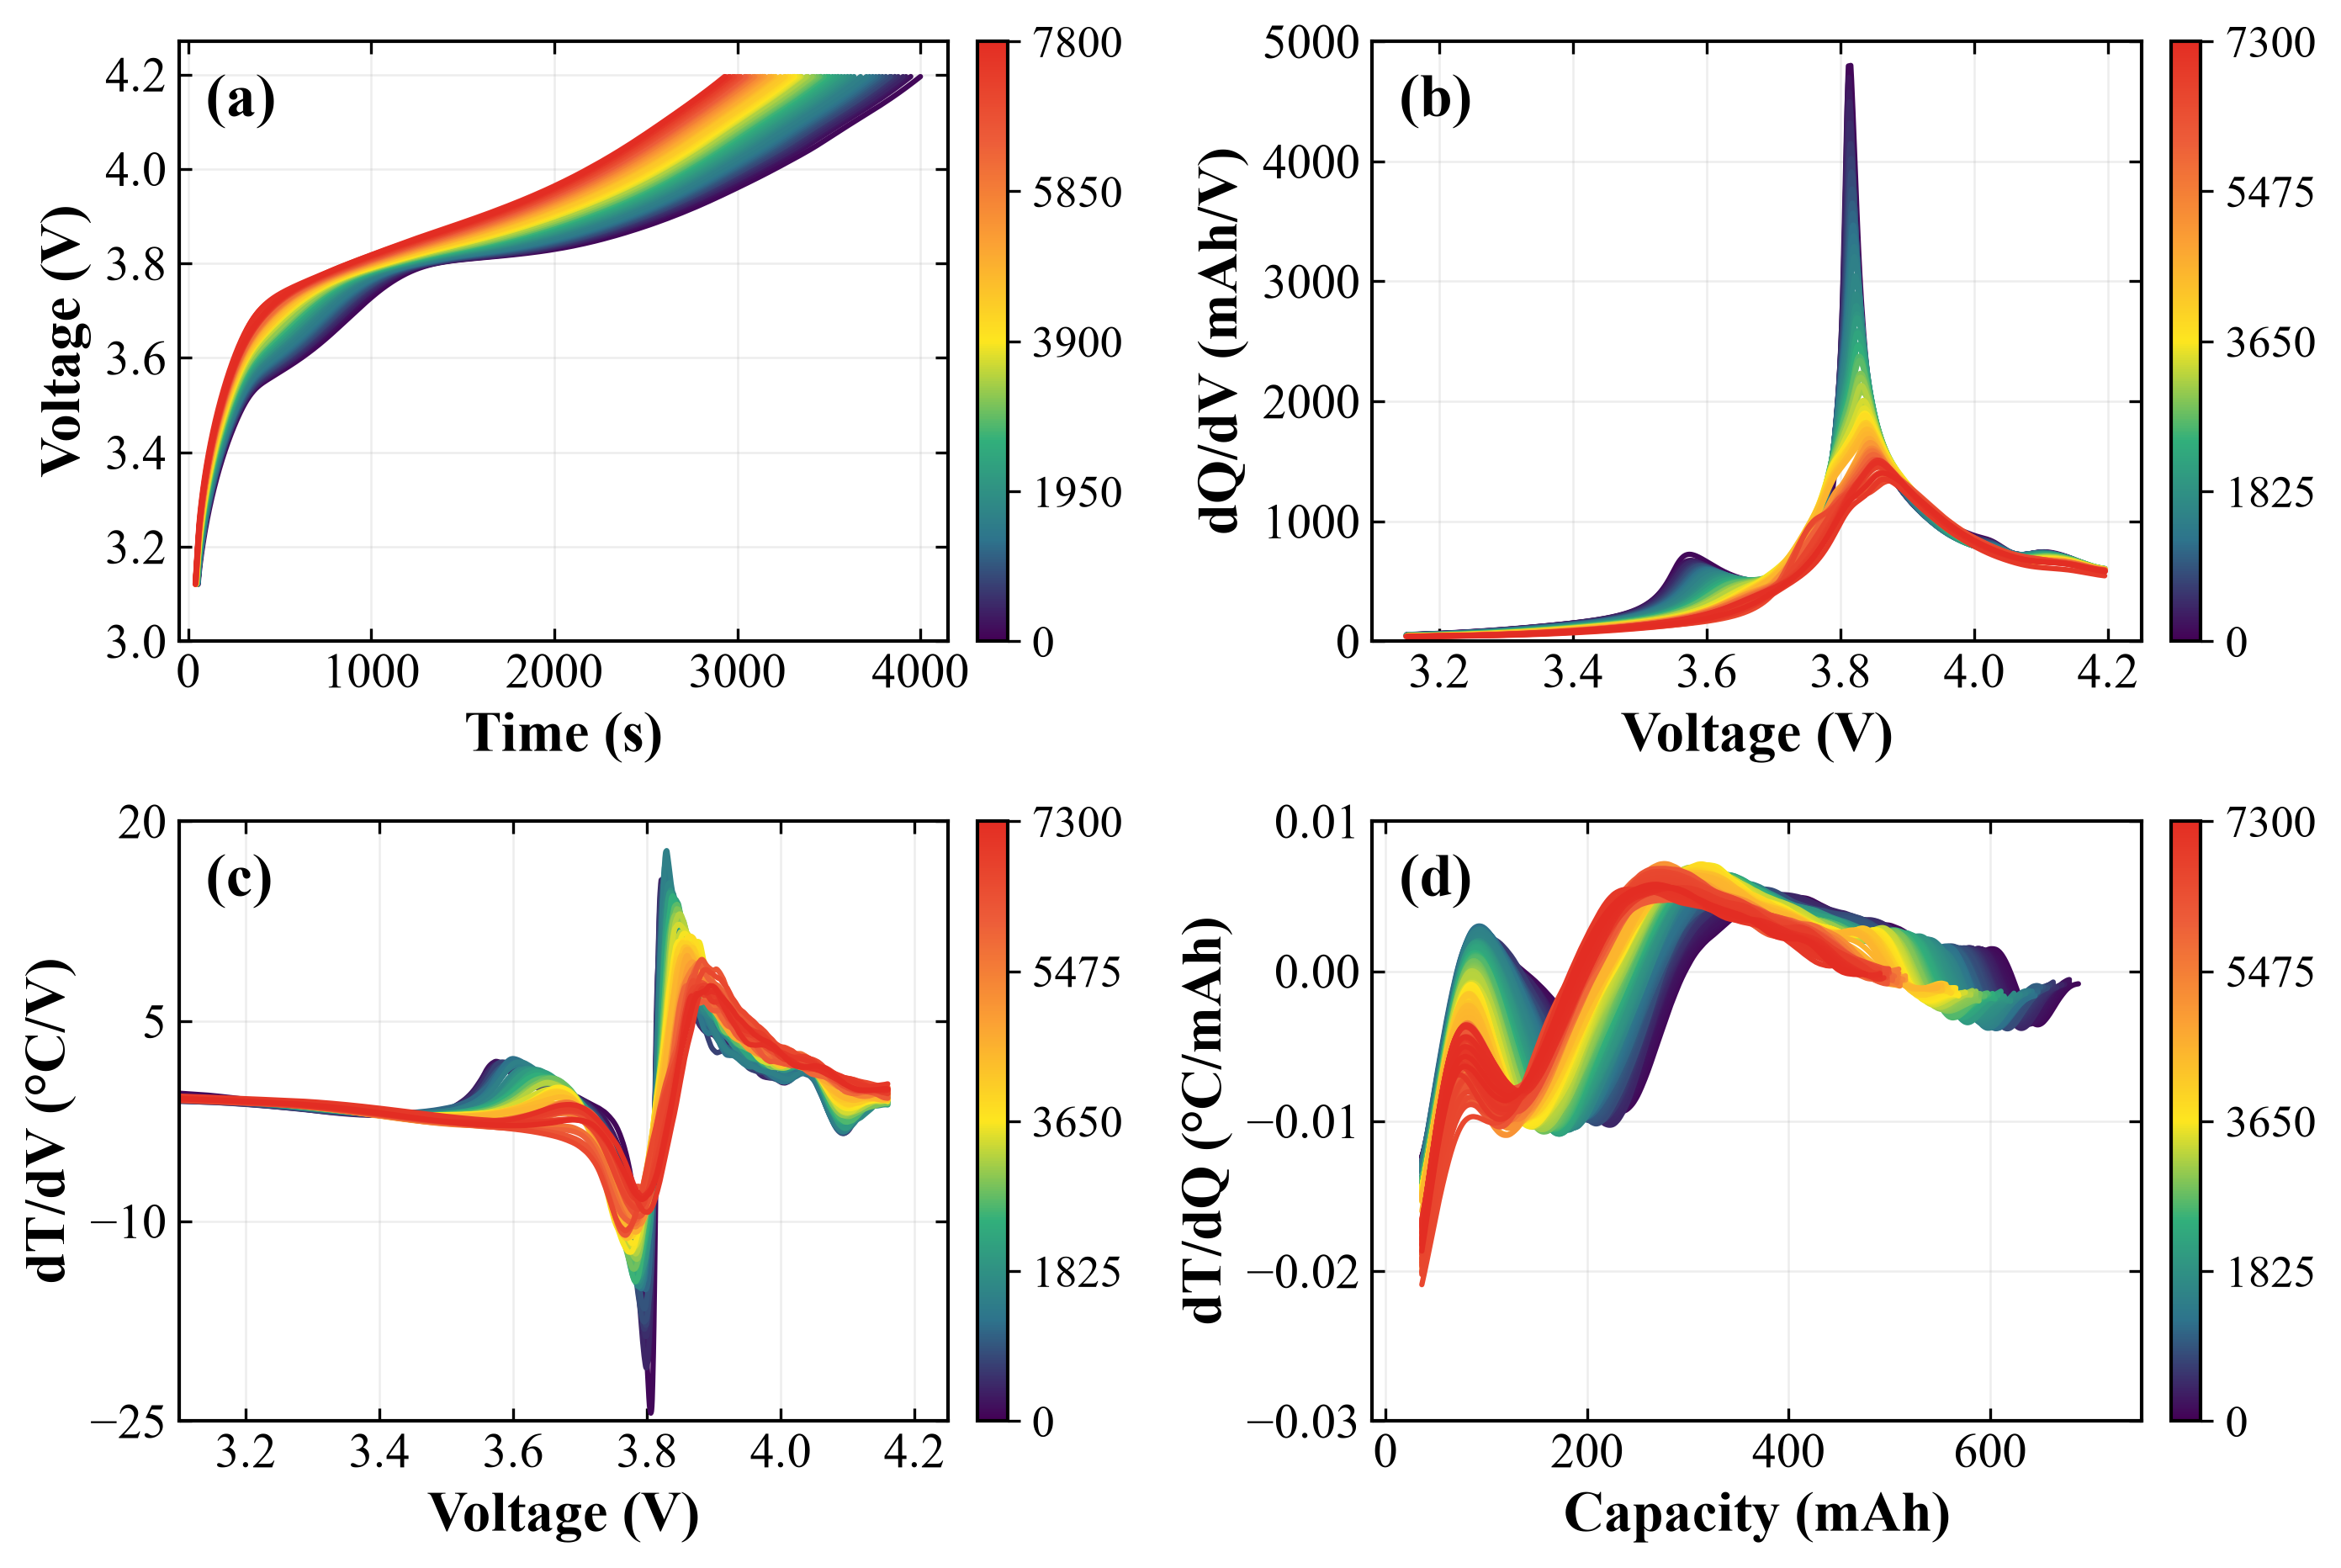
\includegraphics[width=175mm]{figures/fig3.png}%
}
\caption{Charge-side characteristic curves used for candidate HI construction: (a) CVT, (b) IC, (c) DTV, and (d) DTC.}
\label{fig:2-3}
\end{figure}

\FloatBarrier

\subsubsection{Group-Level Dual-Correlation MS-CCCT}
\label{sec:ms-ccct}

Constant current charge time can reflect changes in battery capacity with cycling, but its correlation with SOH depends on the voltage interval used for extraction. Some studies directly extract charging-time features from predefined local voltage intervals\cite{ref28,ref63}. However, degradation-sensitive intervals differ across datasets, and a fixed window used for one dataset is difficult to apply directly to others. To improve the correlation between CCCT and SOH and its stability across cells within the same dataset, this study proposes a group-level dual-correlation multi-scale search method (MS-CCCT). Two cells from the same dataset form the feature-development set $\mathcal{B}$. Correlation results within this set are used to construct a group-level robust score, which determines the extraction window for HI1.

Most existing CCCT window optimization methods use PCC to evaluate candidate intervals\cite{ref31,ref51}. PCC is a common statistical measure of the strength of the linear correlation between CCCT and SOH. However, it is sensitive only to linear changes and is insufficient on its own to characterize monotonic nonlinear relationships. SCC specifically measures monotonic relationships between variables and is suitable for characterizing such nonlinear features. Both PCC and SCC are used to evaluate candidate windows, accounting for the linear correlation and monotonic relationship between CCCT and SOH\cite{ref25,ref55,ref53}. The PCC $\gamma_{i,j}$ and SCC $\rho_{i,j}$ of the $i$th candidate window on the $j$th cell in $\mathcal{B}$ are defined as

\begin{equation}
\gamma_{i,j}=
\frac{\displaystyle\sum_{k=1}^{n_j}(f_{i,j,k}-\bar{f}_{i,j})(y_{j,k}-\bar{y}_j)}
     {\displaystyle\sqrt{\sum_{k=1}^{n_j}(f_{i,j,k}-\bar{f}_{i,j})^2\sum_{k=1}^{n_j}(y_{j,k}-\bar{y}_j)^2}},
\end{equation}

\begin{equation}
\rho_{i,j}=
\frac{\displaystyle\sum_{k=1}^{n_j}\bigl(R(f_{i,j,k})-\bar{R}(f_{i,j})\bigr)\bigl(R(y_{j,k})-\bar{R}(y_j)\bigr)}
{\displaystyle\sqrt{\sum_{k=1}^{n_j}\bigl(R(f_{i,j,k})-\bar{R}(f_{i,j})\bigr)^2\sum_{k=1}^{n_j}\bigl(R(y_{j,k})-\bar{R}(y_j)\bigr)^2}},
\end{equation}

where $f_{i,j,k}$ is the CCCT extracted from the $i$th candidate window at the $k$th cycle of the $j$th cell, $y_{j,k}$ is the SOH of the corresponding cycle, and $n_j$ is the number of valid cycles for that cell. $\bar{f}_{i,j}$ and $\bar{y}_j$ are the mean CCCT and SOH, respectively, and $R(\cdot)$ denotes the ranking operation. Both PCC and SCC range from $-1$ to $1$, with absolute values closer to $1$ indicating stronger correlations.

To account for the correlation performance of each candidate window on both cells, its minimum absolute PCC and minimum absolute SCC within $\mathcal{B}$ are calculated:

\begin{equation*}
mPCC_i=\min_{j\in\mathcal{B}}|\gamma_{i,j}|,\qquad
mSCC_i=\min_{j\in\mathcal{B}}|\rho_{i,j}|.
\end{equation*}

The smaller of these two values is then used as the group-level robust score of the $i$th candidate window:

\begin{equation}
S_i=\min(mPCC_i,mSCC_i).
\end{equation}

This score is determined by the lowest correlation across the two cells, preventing a locally high correlation on a single cell from dominating window selection and allowing the selected window to maintain strong correlations on both cells.

MS-CCCT uses a three-stage coarse-to-fine search. For the Oxford dataset, the initial search range is 3.50--4.20 V. Stage R1 uses a window width of 0.40 V and a step size of 0.20 V for coarse localization, and the window with the highest robust score becomes the search region for the next stage. Stage R2 searches this region using a window width of 0.20 V and a step size of 0.05 V. Stage R3 further refines the search using a window width of 0.10 V and a step size of 0.05 V. If the robust score obtained in R3 exceeds that in R2, the R3 window is selected; otherwise, the R2 result is retained.

For the Oxford dataset, the 3.55--3.75 V window is finally selected with the highest robust score of 0.994447, and its constant current charge time series is used as HI1.

\subsubsection{Health indicator selection}

HI selection is a key step in lithium-ion battery SOH estimation\cite{ref64,ref55}, as the quality of the selected indicators directly affects the final estimation accuracy. Following HI1 window calibration, 15 features based on constant current charge time, IC, DTV, DTC, discharge capacity within a voltage window, and energy efficiency are considered as candidate HIs. Using the same group-level correlation evaluation, PCC and SCC are calculated both between each candidate HI and SOH and between different candidate HIs.

The correlation results for Oxford Cell1 and Cell2 are shown in \cref{fig:2-4}, including both PCC and SCC between candidate HIs and SOH and among the candidate HIs. The lower triangle of each matrix lists the correlation coefficients, while circle size and color in the upper triangle encode correlation strength. Larger, darker circles indicate stronger correlations between the corresponding variables.

The same candidate HI does not show identical correlation performance on the two cells. For HI5 (DTV peak value), the absolute PCC and SCC are 0.949 and 0.966 on Cell1 but decrease to 0.898 and 0.902 on Cell2. In contrast, HI1 maintains high correlations on both cells. Based on the results for Cell1 alone, HI5 would appear to be strongly correlated, but this result does not reflect its correlation level on Cell2. Thus, a correlation ranking based on a single cell cannot fully represent the performance of candidate HIs on other cells.

Existing studies usually select HIs based on the magnitude of their correlation coefficients. When the correlation distributions of candidate HIs change with battery chemistry, operating temperature, or other conditions, the selection results can be sensitive to the data conditions. An indicator that performs well under one condition may become less applicable to other cells or operating conditions. To improve the robustness of HI selection to differences between individual cells and operating conditions, a selection strategy that accounts for the characteristics of correlation distributions is needed.

\begin{figure}[!htb]
\centering
\noindent\makebox[\linewidth][c]{%
  \setlength{\unitlength}{1mm}%
  \begin{picture}(185,181)
    \put(0,0){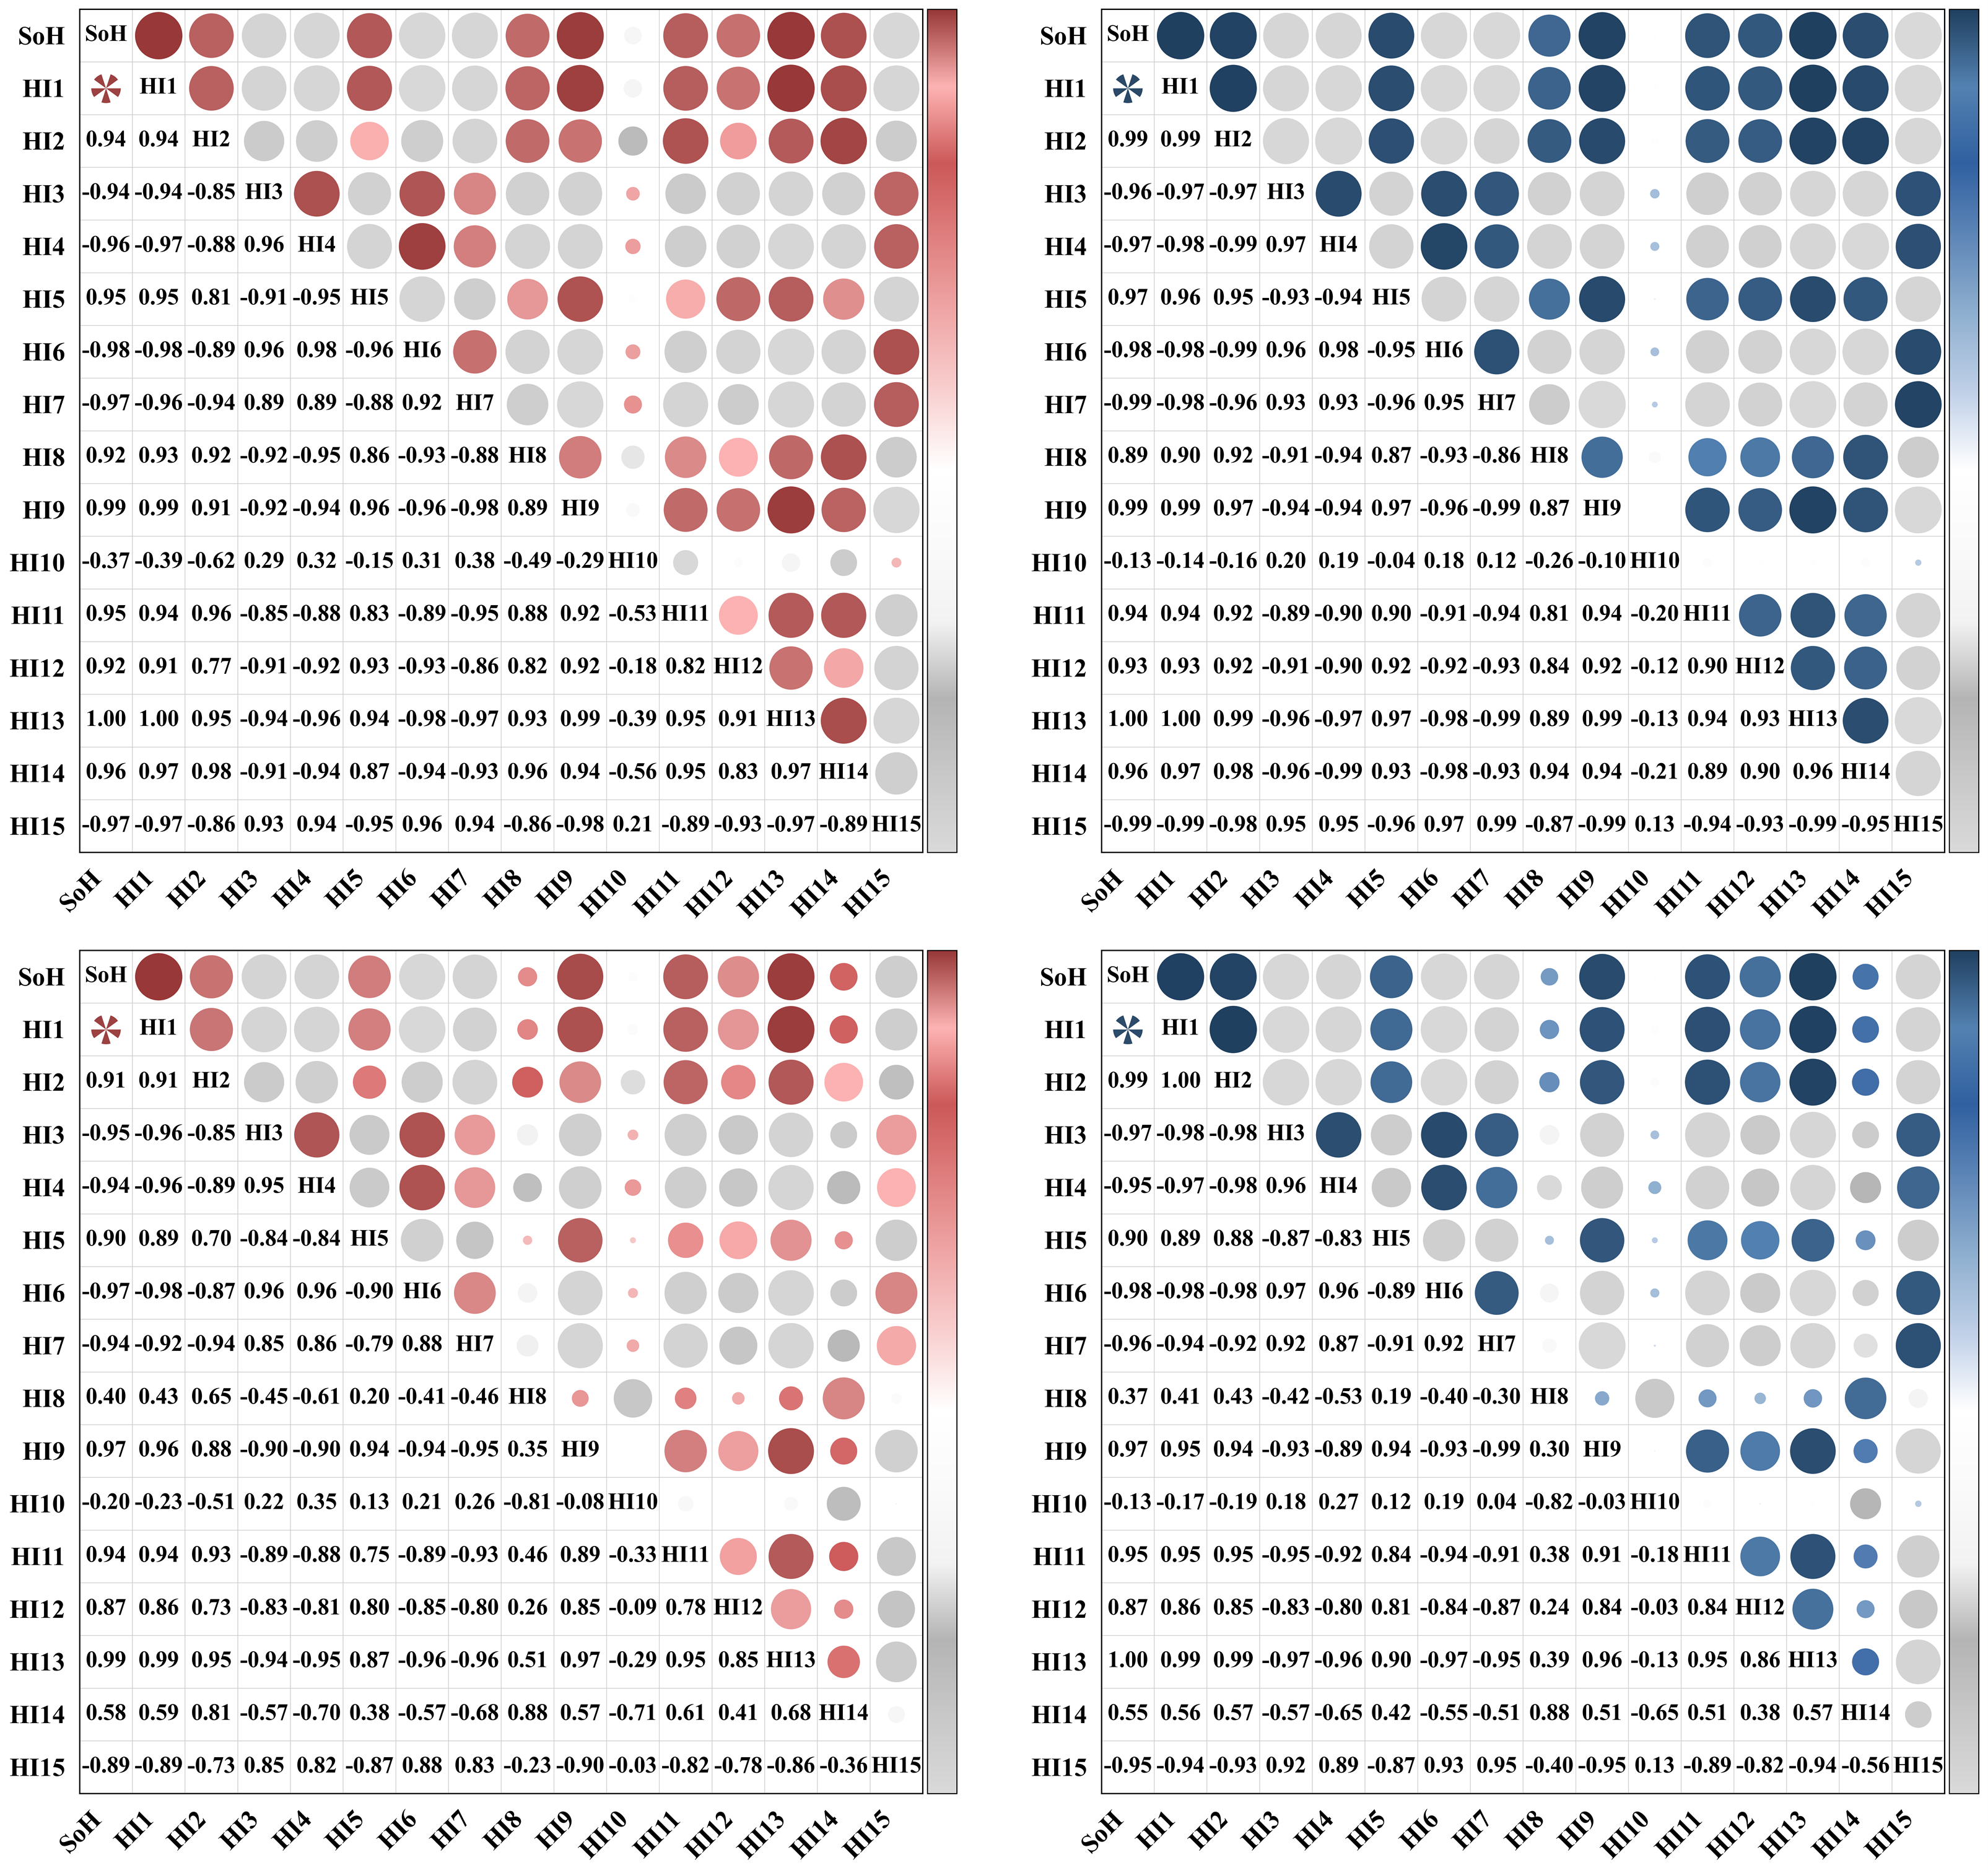
\includegraphics[width=185mm]{figures/fig4_pccscc_print.png}}
    \put(0,177){\makebox(0,0)[l]{\small (a)}}
    \put(98,177){\makebox(0,0)[l]{\small (b)}}
    \put(0,87){\makebox(0,0)[l]{\small (c)}}
    \put(98,87){\makebox(0,0)[l]{\small (d)}}
  \end{picture}%
}
\caption{Correlation matrices of candidate HIs and SOH on the Oxford dataset: (a) Cell1, PCC; (b) Cell1, SCC; (c) Cell2, PCC; (d) Cell2, SCC.}
\label{fig:2-4}
\end{figure}


Accordingly, this study develops a group-level HI selection method. It first considers PCC and SCC on both cells in the feature-development set and retains only candidate HIs that meet all correlation requirements. The correlation matrices also show high correlations between some candidate HIs, indicating redundant information in the candidate pool. The retained HIs are ranked by correlation strength, and features highly correlated with already selected HIs are further removed to reduce redundancy while preserving feature diversity. The specific selection criteria, thresholds, and complete procedure are given in \cref{tab:2-hi-screening-steps}.


After correlation-based admission and redundancy removal, HI1 is retained for the Oxford dataset. Its absolute PCC values on Cell1 and Cell2 are 0.998759 and 0.997322, and its absolute SCC values are 0.998710 and 0.994447, respectively. All four coefficients are close to 1 and differ only slightly between the two cells, indicating that HI1 is highly sensitive to SOH changes during degradation and has good cross-cell consistency.

HI selection is performed only during feature development. Once the indicators are determined, their definitions and calculation parameters remain fixed and are directly applied to feature extraction for the other cells in the corresponding dataset without correlation-based selection, threshold determination, or HI reselection.

With its definition fixed, HI1 achieves absolute PCC values of 0.997874--0.999337 on Cell3--Cell8. Comparisons with existing HIs are presented in \cref{tab:2-hi-literature}. Its correlations exceed the reported values for the listed sample entropy, DTV/IC features, and charging voltage curve slopes on the corresponding cells, showing that HI1 maintains high linear correlations on the remaining six cells.

\input{tables/table_2_hi_screening_steps}
\input{tables/table_2_6}
\FloatBarrier
